\documentclass[12pt]{article}

\usepackage{lmodern}
\usepackage[utf8]{inputenc}
\usepackage[T1]{fontenc}
\usepackage[french]{babel}
\usepackage{url}
\usepackage{graphicx}
\graphicspath{ {./img/} }

\title{\textbf{Analyse de données d’eye-tracking en Réalité Virtuelle}}
\author{\Large{Adonis Stavridis}}
\date{Février 2021}

\begin{document}

% ------------------------------------------------------------------------------
% TITLEPAGE
% ------------------------------------------------------------------------------

\maketitle
\tableofcontents
\pagebreak

% ------------------------------------------------------------------------------
% INTRODUCTION
% ------------------------------------------------------------------------------

\section{Introduction}

L'eye-tracking \cite{wiki:eye_tracking}, ou oculométrie, est une technologie
assez récente qui détermine la position du regard d'un individu dans un
environment virtuel. Elle établie alors une nouvelle interface entre Homme et
machine et c'est devenue aujourd'hui une technologie principale dans des études
liées au système visuel humain, à la psychologie, au marketing et au design.
Elle est aussi dèjà très utilisée dans les jeux vidéos. L'eye-tracking est très
ambitieux, cependant les recherches dans le domaine de la réalité virtuelle
reste encore moindres.

\bigskip
Déterminer la position du regard d'un individu sur un écran permet d'effectuer
des études quantitatives et qualitatives sur de multiples supports, et ainsi
comprendre les comportements humains dans différentes situations. L'eye-tracking
s'avère donc être très pratique pour étudier sur un document par exemple, les
zones qui sont le plus attrayantes et celles qui le sont moins. Cependant,
certaines études ont besoin d'un environment plus réalistes. La réalité
virtuelle ajoute une nouvelle couche d'immersion, permettant à un individu de
se sentir et agir de façon plus réaliste. Ainsi, la réalité virtuelle
permettrait de livrer des résultats beaucoup plus fiables pour certains
domaines, et ainsi pousser à l'avancement des recherches sur le comportement
humain.

\bigskip
En vue de ce travail de recherche, un premier environment a déjà été mis au
point pour recueillir des données d'eye-tracking sur un écran et en réalité
virtuelle. L'objectif est donc de réaliser la visualisation et l'analyse des
données oculaires, en temps réel ou par l'intermédiaire d'une application. Or,
il existe certaines bibliothèques qui permettent de visualiser les données. Donc
laquelle est la plus adaptée pour traiter des données d'oculométrie sur un écran
et en réalité virtuelle?

\bigskip
Il faudrait d'abord comprendre comment sont récupérées les données, quelle est
leur forme et puis énumérer les type de visualisation des données qu'il est
souhaité de réaliser afin de déterminer enfin la bibliothèque la plus
intéressante pour accomplir ce travail d'analyse.

% ------------------------------------------------------------------------------
% CAPTEURS
% ------------------------------------------------------------------------------

\section{Capteurs}

L'eye-tracking est permis grace à des capteurs spéciaux qui envoient des rayons
infrarouges vers les yeux d'un individu. Ils sont infrarouges car ils ne sont
pas visibles par la vision humain. Ces rayons sont alors réfléchis par les yeux
et les capteurs peuvent ainsi déterminer la direction de regard au fil du temps.
Ensuite un logiciel va déterminer la position du regard dans un environment, que
ce soit un écran ou un monde virtuel.

\bigskip
Il existe trois types de capteurs d'oculométrie sur la marché actuellement.
\begin{itemize}
  \item Des capteurs pour écrans : ce sont les capteurs les plus basiques. Ils
        sont placés au-dessus ou en-dessous d'un écran et orientés vers les yeux
        d'un individu. Ils permettent de suivre le regard sur un écran, donc
        dans un environment à deux dimensions.
  \item Des capteurs intégrés à des lunettes : ces capteurs suivent le regard
        d'un individu effectuant des taches dans le monde réel. Les capteurs
        sont alors orientés vers les yeux de l'individu et des caméras capturent
        ce que l'individu observe.
  \item Des capteurs intégrés à des casques de réalité virtuelle : ce sont des
        capteur similaires à ceux des écrans, mais qui ont été manipulés pour
        s'intégrer dans des casques de réalité virtuelle et observer les yeux à
        un distance beaucoup plus courte. Ces capteurs permettraient alors de
        suivre le regard dans un environment à trois dimensions. Un avantage à
        cette technologie ajoutée à la réalité virtuelle est le rendu fovéal
        \cite{wiki:foveated_rendering} : les yeux ne se focalisent qu'en une
        seule région tandis que le reste du champ visuel est flou. Cette méthode
        de rendu propose d'effectuer un rendu de très haute qualité à la région
        de focalisation mais une qualité de rendu moins important dans les reste
        du champ périphérique.
\end{itemize}

\bigskip
La plupart des produits liés à l'eye-tracking sont distribués par des
entreprises telles que Tobii \cite{tobii} et HTC Vice \cite{htc_vive_pro_eye}.
Ces solutions peuvent être utilisés dans plusieurs domaines \cite{yt:tobii_vr}
: les capteurs pour écrans peuvent être utile pour étudier le regard d'un
individu sur une page web, par exemple, et ainsi déterminer les régions les
plus attrayantes ou non. Les lunettes avec capteurs intégrées sont plutôt
utilisés dans le monde professionnel, dans les métiers de l'artisanal, dans la
médicine ou le pilotage. Les casques de réalité virtuelle avec capteurs
intégrés seraient utilisés dans des situations d'entrainement ou des
circonstances pas facilement réalisables dans le monde réel. Certains produits
similaires peuvent aussi être utilisés pour assister à des personnes en
situatio de handicap et à mobilité réduite.

\bigskip
Il existe alors une grande variété des capteurs, certains plus spécialisés dans
des domaines que d'autres, mais ayants le même objectif : suivre le regard. Ce
suivi est d'autant plus utile pour effectuer des recherches. Les capteurs sont
fournis avec des logiciels capables de produire toutes les données nécessaires
pour les analyser.

% ------------------------------------------------------------------------------
% ANALYSE DES DONNÉES
% ------------------------------------------------------------------------------

\section{Analyse des données}

Après avoir récupéré les données brutes d'une séance d'oculométrie, il serait
intéressant des les analyser afin d'en tirer des conclusions pertinantes. Les
données sont une série de nombres, représentants les positions du regard dans un
environment, et sont donc difficilement compréhensibles. Pour cela, il serait
beaucoup plus intéressant de transformer les données en des réprésentations
graphiques de différents types. Il existe différentes mesures et termes
utilisés pour analyser le regard \cite{imotions:metrics}, chacune organisant
les données de façon à avoir une analyse compléte, étudiant tous les aspects du
regard.

\subsection{Points de fixation}

L'un des termes les plus utilisés pour représenter le regard au fil du temps
sont les points de fixation. Ce sont des mesures qui consistent à indiquer
le point de focalisation d'un individu à un instant donné. Un capteur qui
collectionne des données avec un taux d'échantillonage de 120hz, par exemple, va
fournir en sortie 120 points de fixations par seconde. Il faut donc faire une
organisantion des points en fonctions du temps et de l'espace. La quantité de
points de fixations montre à quel point l'attention visuelle a été portée en une
région.

\subsection{Séquence de fixations}

Étudier la séquence de ces points de fixations serait également intéressant. Un
individu va d'abord fixer son regard sur les régions les plus prioritaires et va
se construire l'environment petit à petit, en se concentrant sur différentes
zones. L'ordre d'attention est importante dans la recherche car elle reflète de
l'intérêt d'un individu sur une région et met en avant les objets les plus
captivants au premier regard. Le premier point de fixation peut être aléatoire,
mais les zones de fixations qui suivent peuvent parfois être prédites (pour
une interface utilisateur, par exemple). C'est donc un support qui permet d'en
tirer plusieurs conclusions.

\subsection{Heatmaps}

Une autre représentation très importante est la distribution des points de
fixation, sous la forme d'une heatmap. Un gradient de couleur est placée sur la
environment original indiquant du rouge au bleu les régions les plus
attrayantes (cf. Figure \ref{fig:heatmap}). Ces heatmaps sont un moyen très
simple de séparer les régions les plus attirantes.

\begin{figure}[ht]
  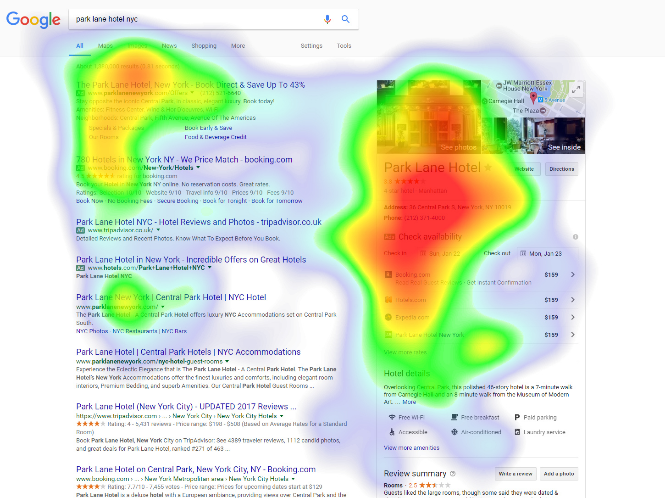
\includegraphics[width=\textwidth,keepaspectratio=true]{heatmap.png}
  \caption{Exemple de heatmap sur une page de recherche sur Google}
  \label{fig:heatmap}
\end{figure}

\subsection{Zones d'intérêt}

Une zone d'intérêt n'est pas vraiment une représentation mais un outil qui
permet de spécifier des zones, des objets au préalable, pour en extraire leurs
mesures. C'est un outil pratique pour bien séparer les différentes zones d'un
environment d'étude, et déterminer les régions les plus importantes. Dans les
mesures de chaque zone, il serait intéressant d'y calculer :

\begin{itemize}
  \item le délai à la première fixation : c'est le temps qu'un individu à mis
        depuis le début pour fixer une zone pour la première fois.
  \item la durée de fixation : c'est la somme du temps qu'un individu a passé a
        fixer une zone
  \item le nombre de fixations : le regard peut fixer une zone, la quitter et
        puis revenir dessus; c'est donc le nombre de fois qu'un individu à fixé
        une zone
\end{itemize}

\bigskip
Il existe donc plusieurs façons d'organiser les données et de les représenter
pour faciliter leur compréhension et permettre d'en tirer les bonnes
conclusions, en prenant en compte tous les aspects de l'étude.

% ------------------------------------------------------------------------------
% LOGICIELS
% ------------------------------------------------------------------------------

\section{Logiciels}

\subsection{GazePointer}

\subsection{Ogama}

\subsection{PyGaze}

\subsection{TurkerGaze}

\subsection{GazeParser}

% De nos jours, la plupart des gens possédent un appareil électronique avec une
% caméra intergrée, que ce soit une webcam ou la caméra d'un smartphone. Il n'est
% pas nécessaire d'acheter du matériel professionnel pour profiter de la
% technologie d'eye-tracking. Il existe plusieurs logiciels et bibliothèques qui
% permettent d'effectuer de l'oculométrie, facilement et gratuitement aussi.

% \subsection{OpenCV}

% L'une des bibliothèques les plus utilisées dans le traitement d'images en temps
% réel et en vision par ordinateur ou Computer Vision est OpenCV \cite{opencv}.
% Elle propose des fonctionnalités pour traiter des données brutes d'images, mais
% aussi une grande variété d'outils issus de l'état de l'art en vision des
% ordinateurs (détection de visage par exemple) et des algorithmes d'apprentissage
% artificiel. En tout, c'est une bibliothèque très compléte, pour la majorité des
% domaines de la vision par ordinateur, mais pas forcément spécialisée dans
% l'oculométrie. Il est possible toutefois d'écrire des algorithmes pour suivre
% le regard grace aux outils mis à disposition par la bibliothèque. Il existe
% également de jeux de données assez grands mis à disposition en ligne, tel que
% NVGaze \cite{nvgaze} de NVidia, pour entrainer des réseaux de neurones à
% éstimer le regard grace à des images \cite{gaze_tracking}. OpenCV propose plein
% d'outils de visualisation des données en temps réel, mais aucun pour leur
% exploitation.

% \bigskip
% Le grand avantage de OpenCV est son age et popularité. Elle est la bibliothèque
% de référence dans le domaine de la vision par ordinateur, propose parmi des
% outils très optimisés, tout en restant bien documenté. C'est aussi un projet
% open-source, et c'est pour cela qu'elle rassemble une grande communauté.
% Puisqu'elle n'est pas spécialisée dans l'eye-tracking, elle ne propose pas
% d'outils d'analyse et de visualisation de données, nécessaires en oculométrie.

% \subsection{PyGaze}

% Une autre bibliothèque très intéressante est PyGaze \cite{pygaze}. C'est une
% toolbox permettant de suivre le regard sur un écran grace à une caméra ou
% webcam. Elle propose également des outils pour analyser les données
% enregistrées, lors d'une séance d'eye-tracking. Ces outils permettent de créer
% plusieurs types d'images pour suivre le regard au fur et à mesure du temps.
% Parmi ces images se trouvent des cartes de fixations, des heatmap et des schémas
% du chemin du regard. Elle permettent de facilement comprendre les données et
% d'en tirer des conclusions plus rapidement. En plus, la bibliothèque PyGaze peut
% être utilisée avec la SDK de Tobii pour profiter de toutes les fonctionnalités
% des produits Tobii.

% \bigskip
% Cette bibliothèque est donc idéale pour visualiser les données récupérées grace
% àl'oculométrie, de façon simple et efficace. Cette libraire est assez bien
% documentée aussi. PyGaze est donc vraiment intéressante à utiliser, en
% combinaison avec les capteurs Tobii pour tirer profit d'un maximum de données
% et créer des images de synthése les plus concluantes possibles. Ces-dernieres
% sont très importantes pour permettre de tirer les bonnes conclusions.



\begin{itemize}
  \item https://imotions.com/blog/10-terms-metrics-eye-tracking/
  \item https://www.gazept.com/product/gazepoint-analysis-professional-edition-software/
  \item https://imotions.com/blog/free-eye-tracking-software/
\end{itemize}

% ----------------------------------------------------------------------------
% CONCLUSION
% ----------------------------------------------------------------------------

\section{Conclusion}

% ----------------------------------------------------------------------------
% BIBLIOGRAPHIE
% ----------------------------------------------------------------------------

\pagebreak
\bibliographystyle{unsrt}
\bibliography{recherches}

\end{document}
